% --- Il metodo -- %

\begin{tframe}{Il metodo}

\vspace{0.5cm}
Il metodo proposto è suddiviso nelle seguenti fasi:
\vspace{0.5cm}
\begin{itemize}
\item Estrazione dei \textbf{PRNU} dalle immagini
\vspace{0.5cm}
\item Calcolo della \textbf{matrice dei pesi} tramite \textbf{PCE}
\vspace{0.5cm}
\item \textbf{Clustering} delle immagini (usando \emph{Normalized Cuts})
\vspace{0.5cm}
\item Generazione delle \textbf{fingerprints} di camera
\end{itemize}
\end{tframe}


\begin{tframe}{PRNU}

Il \textbf{PRNU}, \emph{Photo-Response Non-Uniformity}, è un rumore di tipo \emph{pattern noise} presente nelle immagini, dovuto principalmente dal tipo di sensore utilizzato e da difetti in fase di costruzione.

\vspace{0.3cm}

Il PRNU si scompone in:
\vspace{0.5cm}
\begin{itemize}
\item \textbf{Pixel Non-Uniformity} (\textbf{PNU}): risultante dalla differenza di luminosità dei pixels in regioni non omogenee e imperfezioni del sensore
\item Componenti a bassa frequenza
\end{itemize}

\vspace{0.5cm}
In generale, due immagini acquisite dallo stesso sensore CCD presentano lo stesso rumore PNU.

\end{tframe}


\begin{tframe}{Clustering}

L'operazione di \textbf{clustering} consiste nel raggruppare elementi (immagini) tra loro \emph{simili} in gruppi tra loro disgiunti.

\vspace{0.5cm}

\textbf{Similarità}: due immagini sono tra loro simili se la loro \textbf{Peaks-to-Correlation Energy} (\textbf{PCE}) è alta.

\vspace{0.7cm}

Viene dunque costruita una \emph{matrice di similarità} $w$ tra le immagini il cui generico elemento

$$
w(i, j) = PCE(PRNU_i, PRNU_j)
$$

\end{tframe}

\begin{tframe}{Clustering}

Il clustering è infine eseguito dall'algoritmo \textbf{Normalized Cuts}.
\vspace{0.3cm}

Dato un \emph{grafo pesato} $G = <V, E>$, i cui pesi associati agli archi sono definiti nella matrice $w$, procede ricorsivamente bipartizionando il grafo $G$ ad ogni passo in due sottografi $A$ e $B$ (con $A \cup B = V$ e $A \cap B = \varnothing$). Per ciascuna bipartizione calcola un \emph{valore del taglio
}
$$
cut(A, B) = \sum_{u \in A, v \in B} w(u, v)
$$

Il taglio ottimale per partizionale il grafo è calcolato ottimizzando il valore di un \textbf{taglio normalizzato}

$$Ncut(A, B) = \frac{cut(A, B)}{assoc(A, V)} + \frac{cut(A, B)}{assoc(B, V)}$$

\end{tframe}



\begin{tframe}{Estrazione delle \emph{fingerprints}}

Eseguito il clustering delle immagini, per ciascun cluster viene generata una \textbf{fingerprint} a partire dalle immagini in esso contenute.

\begin{figure}[h]
\begin{center}
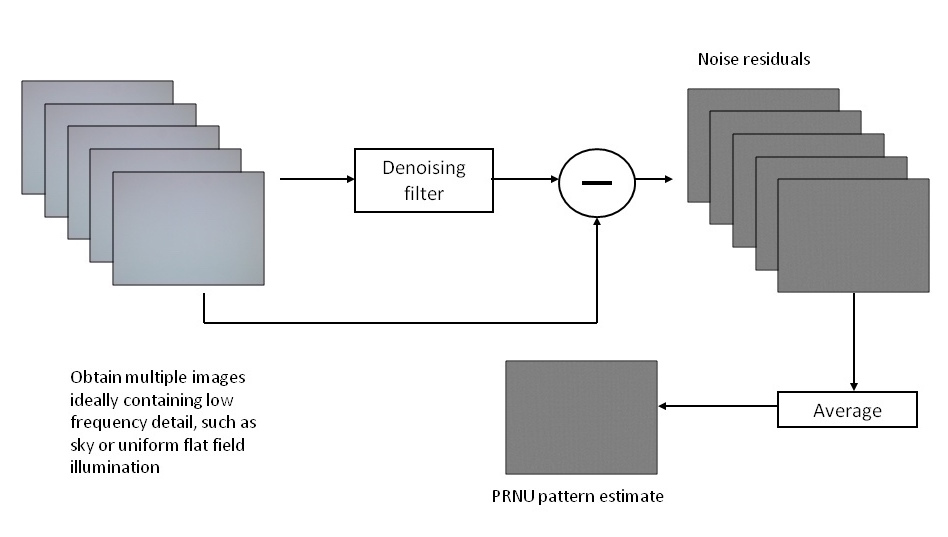
\includegraphics[width=0.8\textwidth]{../images/prnu_extraction_2}
\end{center}
  \caption{Estrazione della \emph{fingerprint} da ciascun cluster ottenuto}
\label{fig:soglia AC}
\end{figure}
\end{tframe}